\documentclass{article}
\usepackage[english]{babel}

\usepackage[letterpaper,top=2cm,bottom=2cm,left=3cm,right=3cm,marginparwidth=1.75cm]{geometry}

\usepackage{graphicx}
\graphicspath{ {./images/} }

\title{HW 1 Report}
\author{Han Xie}

\begin{document}
\maketitle
Group Member: Gengyao Qiu, Manish Chandra Karumuri

\section{Project Description}
In this project we have been successfully build the python project with makefile. The python file trignometry.py is able to plot the trignometry function as user input, read the txt file user input, and also write and print based on user decision. The figure below is one example of what the Python file is able to do.

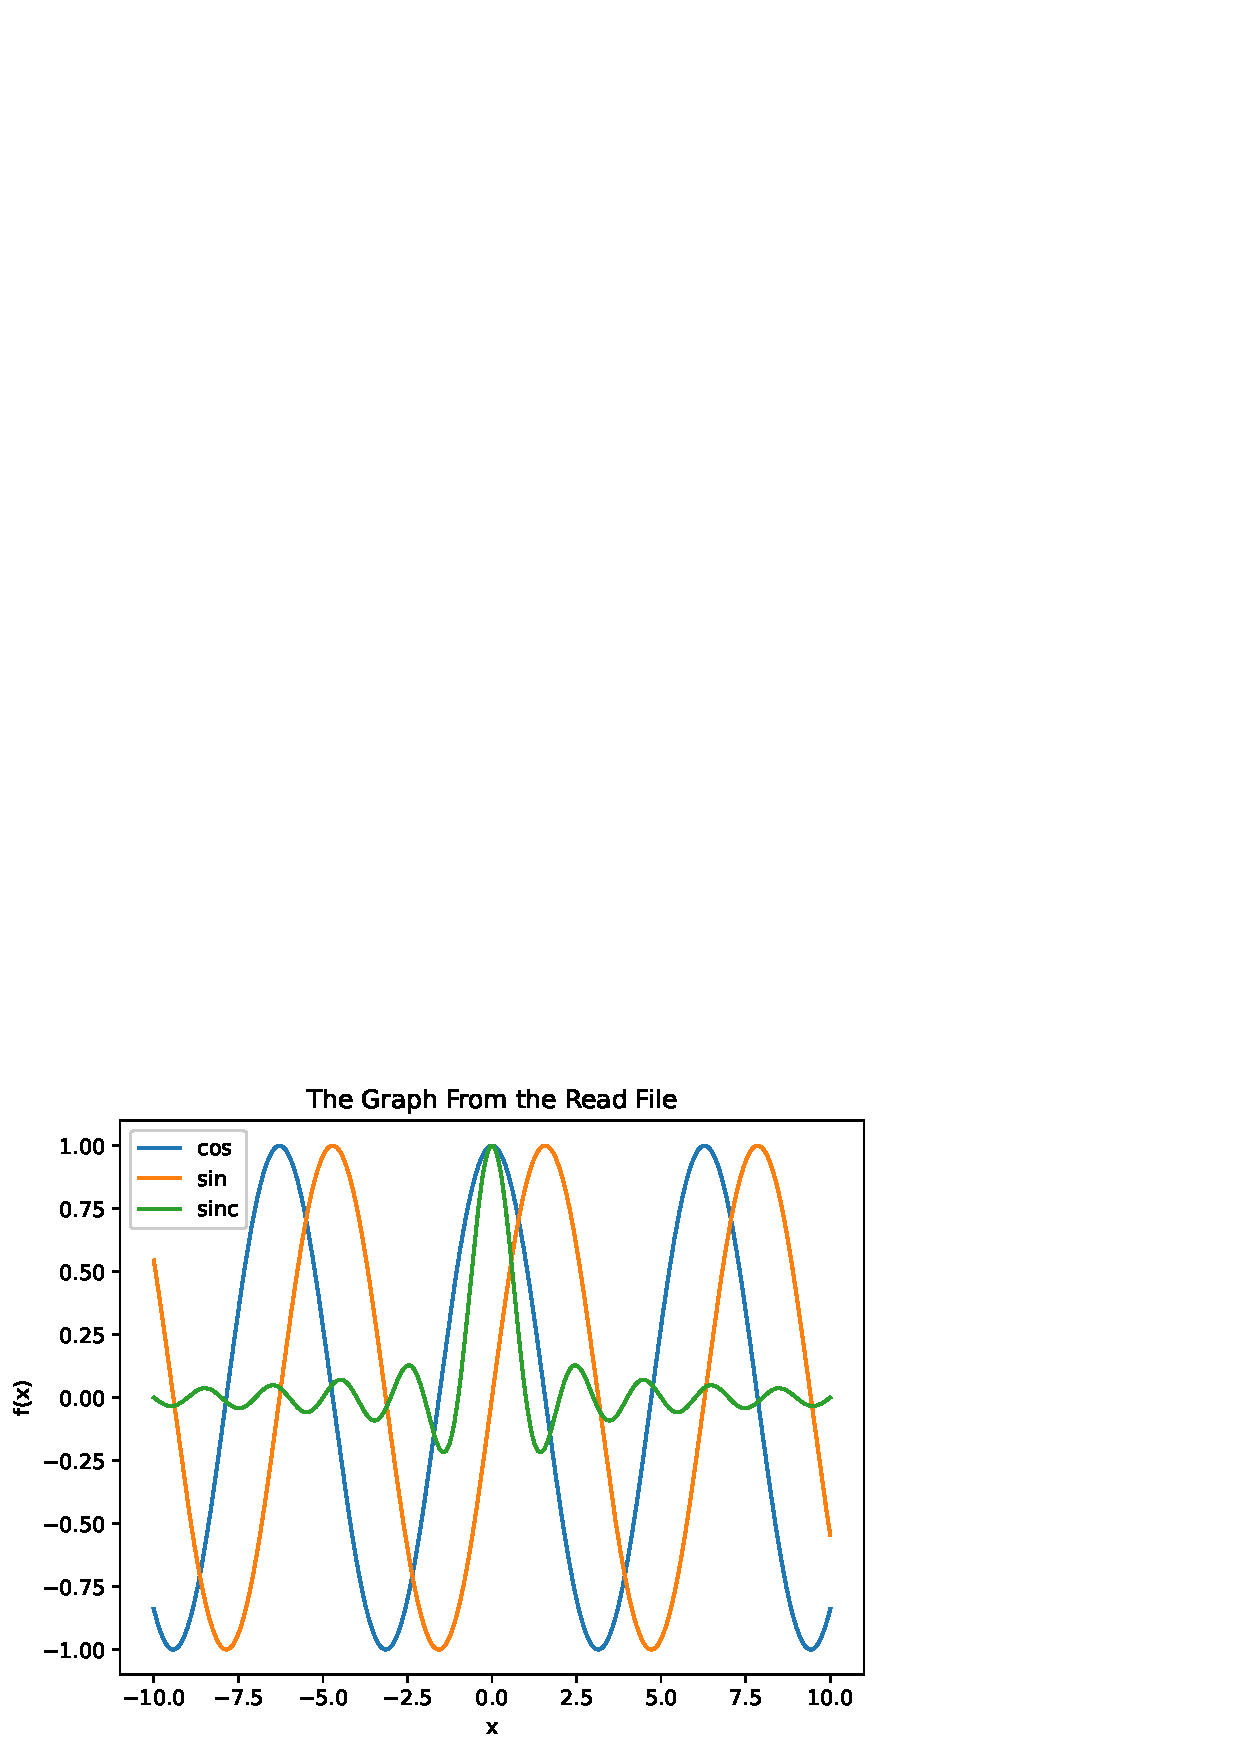
\includegraphics{read_file_figure.jpeg}

\section{Contribution}
Our group contributes equally. We have groupmates ask questions and being solved by other groupmates. We create a positive learning and coding environment.

\end{document}
